
%(BEGIN_QUESTION)
% Copyright 2015, Tony R. Kuphaldt, released under the Creative Commons Attribution License (v 1.0)
% This means you may do almost anything with this work of mine, so long as you give me proper credit

Calculate the current passing through this 87 relay's operate coil (87/OC) given the two currents sent through the restraint coils (87/RC):

$$\includegraphics[width=15.5cm]{i02607x01.eps}$$

$I_{RC1} = 4.72 \hbox{ A} \> \angle 21^o$

\vskip 10pt

$I_{RC2} = 4.68 \hbox{ A} \> \angle -160^o$

\vskip 10pt

In addition to calculating a symbolic answer for $I_{OC}$, sketch a phasor diagram showing how the three currents ($I_{RC1}$, $I_{RC2}$, and $I_{OC}$) relate to one another.


\vskip 20pt \vbox{\hrule \hbox{\strut \vrule{} {\bf Suggestions for Socratic discussion} \vrule} \hrule}

\begin{itemize}
\item{} Identify factors which could account for these two currents not perfectly canceling each other at the differential current relay.
\end{itemize}

\underbar{file i02607}
%(END_QUESTION)





%(BEGIN_ANSWER)


%(END_ANSWER)





%(BEGIN_NOTES)

Applying Kirchhoff's Current Law at the node where these three currents intersect:

$$I_{OC} = I_{RC1} + I_{RC2}$$

$$I_{OC} = (4.72 \hbox{ A} \> \angle 21^o) + (4.68 \hbox{ A} \> \angle -160^o)$$

$$I_{OC} = 91.26 \hbox{ mA} \> \angle 84.5^o$$

$$\includegraphics[width=15.5cm]{i02607x02.eps}$$

%INDEX% Electronics review, phasor expressions of circuit quantities
%INDEX% Protective relay: differential current (87)

%(END_NOTES)


